\section{Macro areas}

\begin{figure}[H]
  \centering
  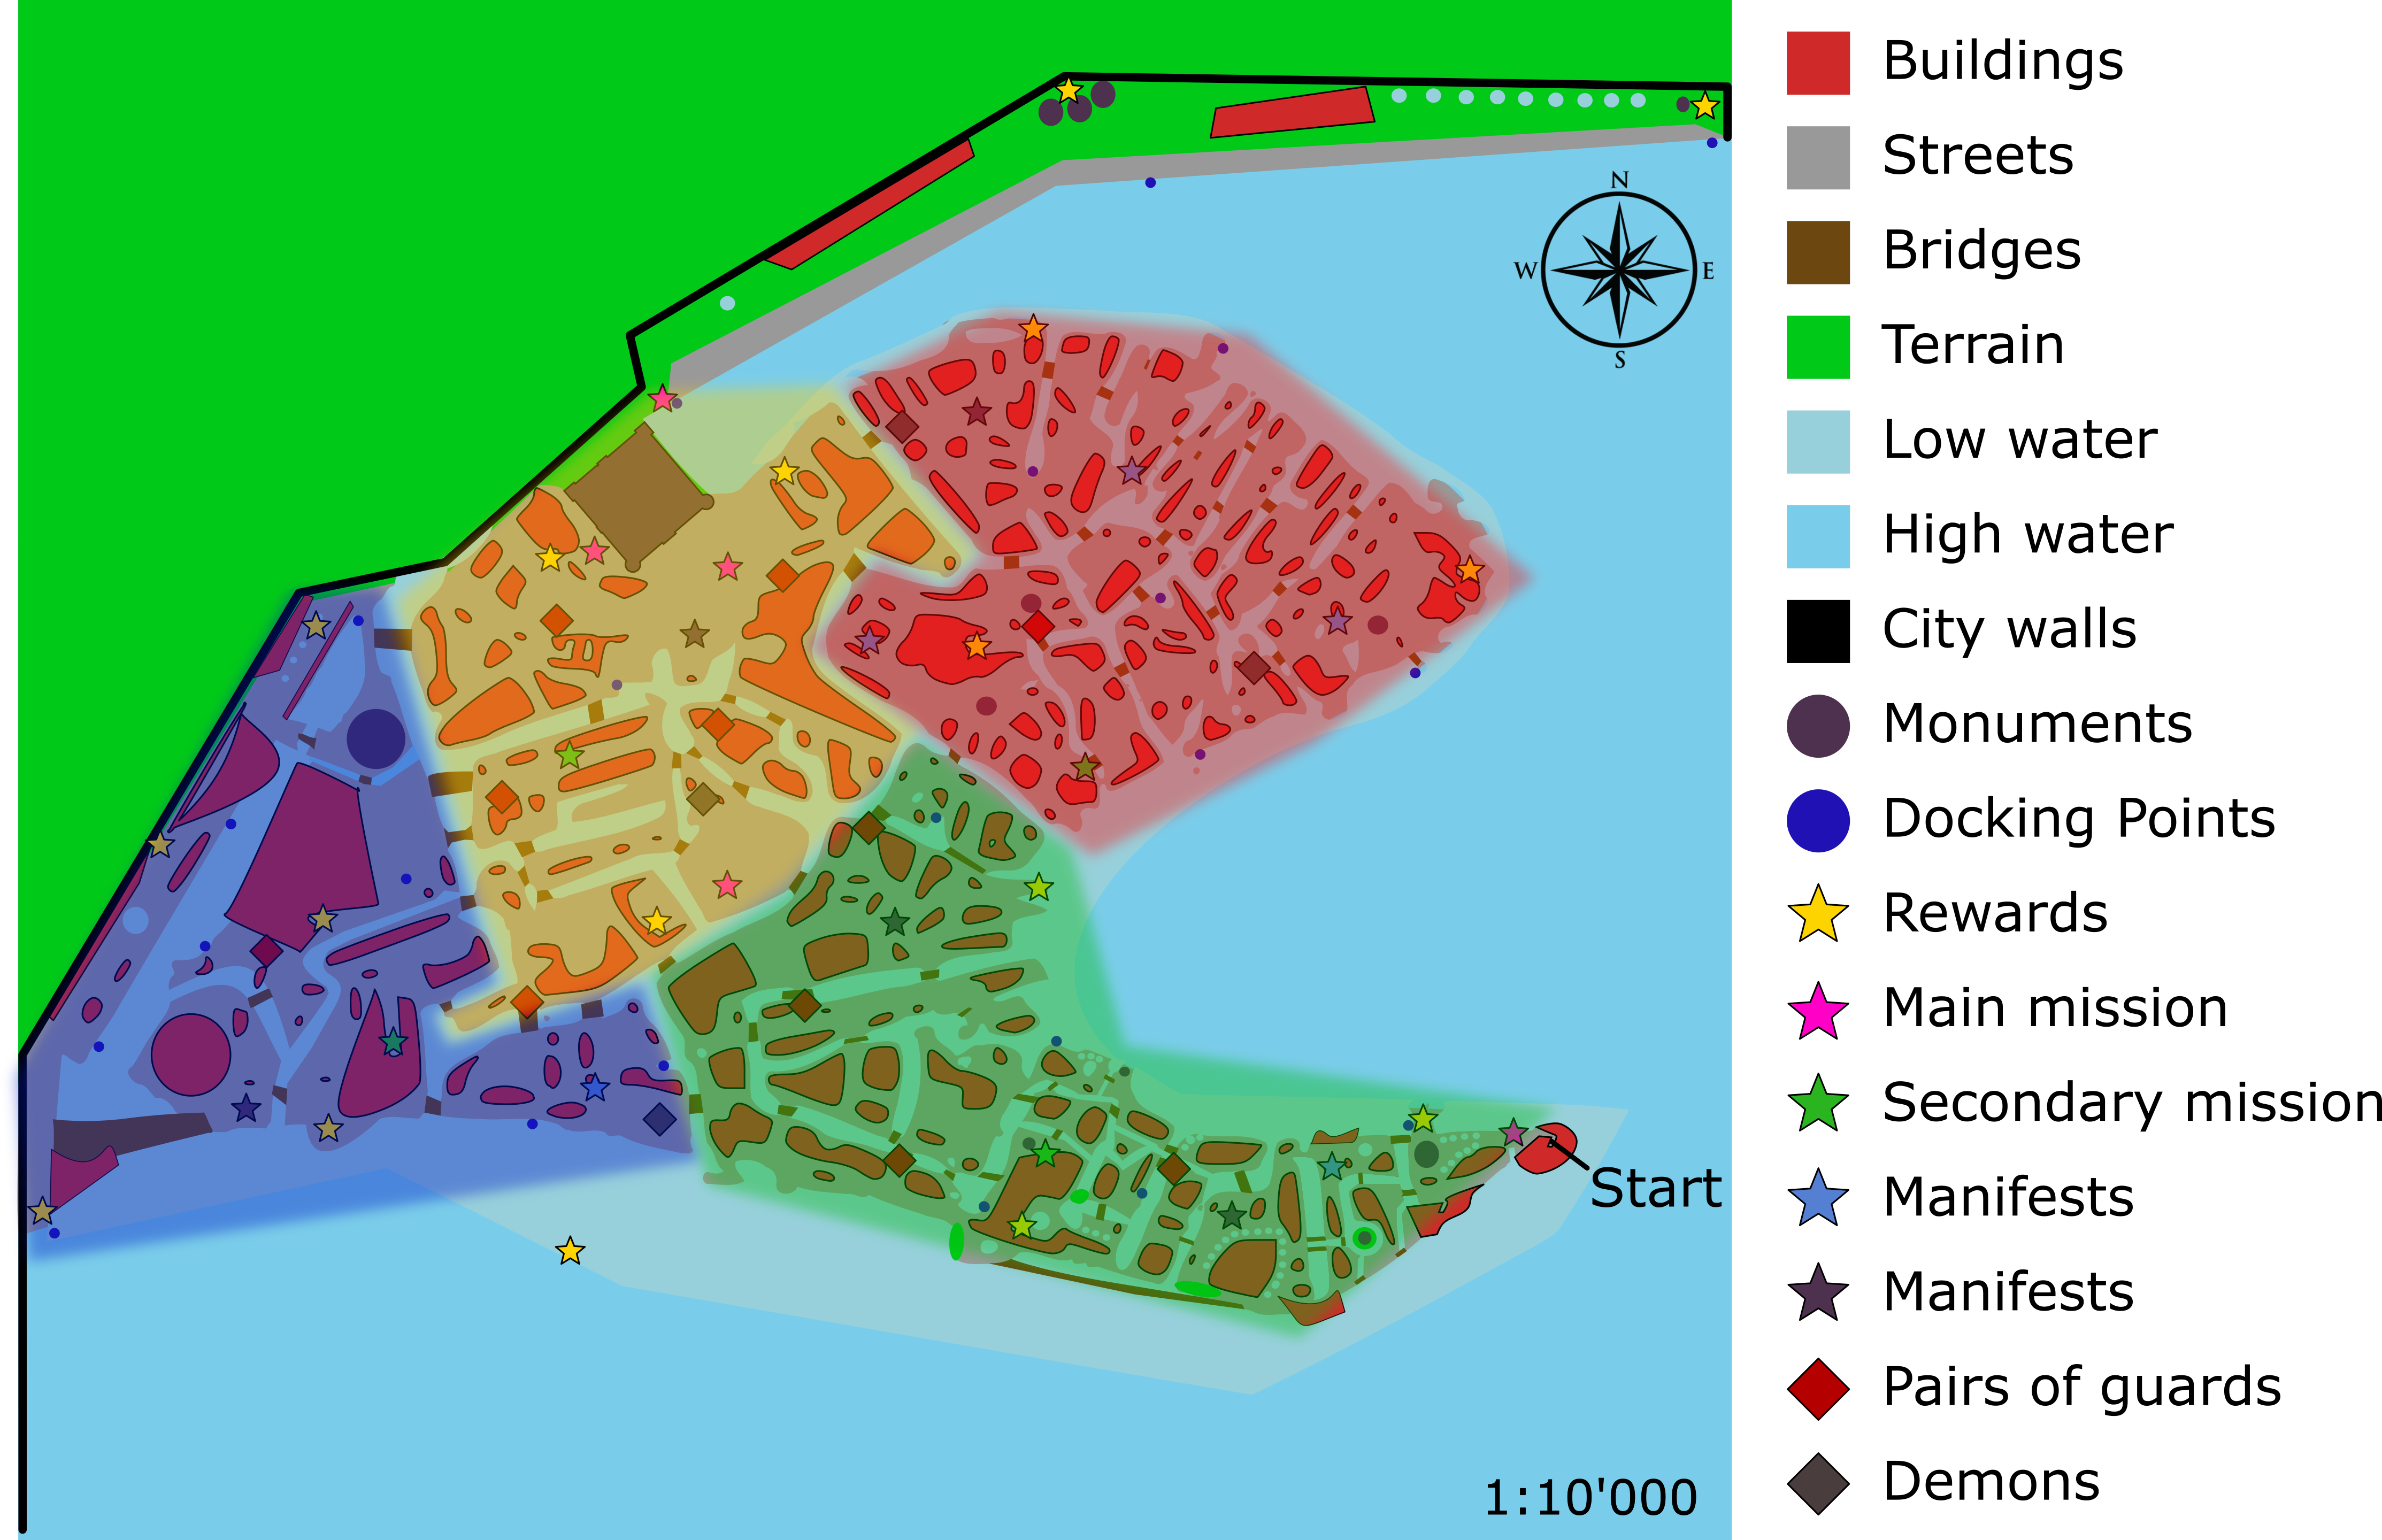
\includegraphics[width=\textwidth]{Images/Maps/dynamiaAreas}
  \caption{Macro areas of Dynamia}
\end{figure}

\subsection{Southern area (green)}
This is the first area that the player will see.

The southern area is the newest part of Dynamia and it is very dynamic. People who come from outside the city has chosen this area to build their house, in the outskirts of the city. Here it is common to see every kind of people from every part of the region and we can find a mix of cultures and languages. The high triumph arc in the end of the city can be seen from the sea and it is a \enquote{welcome} for all of the people who reach Dynamia.

\begin{figure}[H]
  \centering
  
\includegraphics[width=6cm]{Images/Palettes/dynamiaSouthernArea}
  \caption{Palette for the southern area of Dynamia}
\end{figure}

\subsection{Central area (yellow)}
This is by far the richest area in the city. In fact here we can find the houses of  nobles and rich merchants as well as the castle and the market. Given this, here is common to find jewelries, merchants who sell luxury items and highly decorated villas on the canals.

In addition to the castle and the market that will be described in next paragraphs, another important landmark is the square in front of the castle itself. Here from early morning till evening, newsboys scream and shout trying to sell their newspapers to the people who pass by or to simply announce the new rules and laws that the queen has issued.

In this area there are more guards and demons than in the other parts of the city. People's clothes are very fashionable and expensive. Most of the boats in the canals are elegant rowboats or quiet and modern steam-powered ships.

\begin{figure}[H]
  \centering
  
\includegraphics[width=6cm]{Images/Palettes/dynamiaCentralArea}
  \caption{Palette for the central area of Dynamia}
\end{figure}

\subsection{Harbor area (blue)}
The harbor occupies the western area of the city. On the large canal near the city walls we can find a huge freight yard and some shipyards, the  other buildings in this zone are mostly houses of fishermen and warehouses.

This area is the main door on the sea of the city and allows big ships to enter into the city to drop off their supply or get repaired before heading to the open sea. Here we can find both the biggest bridge and the biggest monument of Dynamia. The bridge is a drawbridge that opens up to let cargo ships get in, while the monument represents the Goddess of Fortune and here merchants and fishermen come to pray before they set sail.

Here the canals are very busy, in particular there are a lot of steam-powered ships that take the goods to the rest of the city. Most of the people in this area are fishermen or workers in the harbor and they wear work clothes.

\begin{figure}[H]
  \centering
  
\includegraphics[width=6cm]{Images/Palettes/dynamiaHarborArea}
  \caption{Palette for the harbor area of Dynamia}
\end{figure}

\subsection{Ghetto area (red)}
The ghetto area is called this way because, centuries before, it was the area where  minorities where confined. Nowadays it has changed, but it is still a depraved area where you can find travelers and people who can't afford something better, but even some middle-class folks.

The streets are typically more crowded and dirtier; houses are not as elegant as in the center, generally built with only wood or concrete and without any sort of decoration.

We can find some little shops who sell fresh food and bread, some little factories and few handicraft workshop. So, differently from the scent of rare spices from the southern desert we can smell in the central area, here we can find only the smell of fish and smoke.

In this area there are only a few guards and demons. People's clothes are dirty, worn out and full of patches. Most of the boats are old rowboats or old steam-powered ships that make a lot of black smoke.

\begin{figure}[H]
  \centering
  
\includegraphics[width=6cm]{Images/Palettes/dynamiaGhettoArea}
  \caption{Palette for the ghetto area of Dynamia}
\end{figure}
